\section{Graphical Models} 

  The concept of using latent variables to model some process will be used over and over again. We have seen simple examples of latent linear models, but what about nonlinear ones? It turns out that these can be seen as a specific instance of \textit{graphical models}. 

  When computing high-dimensional distributions, the parameters needed to encode this density scales badly. We can see that a general Gaussian mixture model in $\mathbb{R}^n$ with $k$ clusters requires $O(n^2 k)$ parameters. If we wanted to sample from a distribution of portraits, then the dimension $n$ would be the resolution of the image. For a $1024 \times 1024$ image, this requires $n = 3 \cdot 2^{20}$ dimensions, and modeling it with a GMM is hopeless. Fortunately, for complex distributions there is usually some dependencies (e.g. between neighboring pixels) that we can take advantage of. This is exactly what graphical models do. They factor complex distributions so that the scaling is much better. While there are graphical models that do not use latent variables, most interesting applications of graphical models require latent variables, and so we will focus on that. Additionally, we will introduce the EM algorithm, which will be used repeatedly and is particularly important in optimizing \textit{variational autoencoders} in deep learning. 

\subsection{Bayesian Networks (Directed Graphical Models)} 

  Note that the whole purpose of directed graphical models is to model some sort of \textit{causal} relationship between two random variables. Note that while this is successful in practice, there is really no way to know for sure about any causality. 

  \begin{definition}[Bayesian Network]  
    A \textbf{Bayesian network}, also known as a \textbf{directed probability model}, is a directed acyclic graph of $M$ nodes representing a joint probability distribution of $M$ scalar random variables. An edge pointing $A \rightarrow B$ means that the $B$ is conditionally dependent on $A$, and that there is a very clear casual relationship coming from $A$ to $B$. The \textbf{parents} of a node $x_i$ is denoted $\mathrm{pa}_i$, and the entire joint distribution can be broken up as such: 
    \begin{equation}
      p(\mathbf{x}) = \prod_{m=1}^M p(x_m \mid x_{\mathrm{pa}_m})
    \end{equation}
    which is unique due to it being a DAG. Not only is a Bayesian network easy to parameterize. We can also sample from the joint distribution by sequentially sampling starting from the parents to the final children, and discarding the ones (marginalizing) that we don't wish to sample. This is known as \textbf{ancestral sampling}. 

    \begin{figure}[H]
      \centering 
      \begin{tikzpicture}[node distance=2cm]
        \node [node_style] (x1) at (0,0) {$x_1$};
        \node [node_style] (x2) at (-1,-1.5) {$x_2$};
        \node [node_style] (x3) at (1,-1.5) {$x_3$};
        \node [node_style] (x4) at (0,-3) {$x_4$};
        
        \draw [edge_style] (x1) -- (x2);
        \draw [edge_style] (x1) -- (x3);
        \draw [edge_style] (x2) -- (x4);
        \draw [edge_style] (x3) -- (x4);
        
        \node [above=0.2cm of x1] {Root Node};
        \node [below=0.2cm of x4] {Child Node};
      \end{tikzpicture}
      \caption{} 
      \label{fig:bayesian_network}
    \end{figure}
  \end{definition}

  This following example cleared up any confusion when I learned Bayesian networks for the first time. 

  \begin{example}[Relay Race]
    Consider a $4\times100$m relay race where the final race time depends on multiple factors. We can model this as a Bayesian network where the total race time $T$ depends on:
    \begin{itemize}
      \item Individual runner capabilities ($R_1$, $R_2$, $R_3$, $R_4$)
      \item Handoff success between runners ($H_1$, $H_2$, $H_3$)
      \item Individual leg performances ($P_1$, $P_2$, $P_3$, $P_4$)
    \end{itemize}

    The joint probability distribution factorizes as:
    \begin{align*}
      & p(T, R_1, R_2, R_3, R_4, H_1, H_2, H_3, P_1, P_2, P_3, P_4) = \\
      & p(T|P_1,P_2,P_3,P_4) \prod_{i=1}^4 p(R_i) \prod_{i=1}^3 p(H_i|R_i,R_{i+1}) \prod_{i=1}^4 p(P_i|R_i,H_{i-1})
    \end{align*}

    \noindent where $H_0$ is undefined for $P_1$, and each runner's performance depends on their capability and the success of the previous handoff (except for the first runner). This network captures both the individual contributions and the critical dependencies between runners during baton exchanges.

    \begin{figure}[H]
      \centering 
      \begin{tikzpicture}[node distance=2cm]
        % Runner nodes
        \node[runner_node] (r1) at (0,0) {$R_1$};
        \node[runner_node] (r2) at (2,0) {$R_2$};
        \node[runner_node] (r3) at (4,0) {$R_3$};
        \node[runner_node] (r4) at (6,0) {$R_4$};
        
        % Handoff nodes
        \node[factor_node] (h1) at (1,-1.5) {$H_1$};
        \node[factor_node] (h2) at (3,-1.5) {$H_2$};
        \node[factor_node] (h3) at (5,-1.5) {$H_3$};
        
        % Performance nodes
        \node[factor_node] (p1) at (0,-3) {$P_1$};
        \node[factor_node] (p2) at (2,-3) {$P_2$};
        \node[factor_node] (p3) at (4,-3) {$P_3$};
        \node[factor_node] (p4) at (6,-3) {$P_4$};
        
        % Final outcome
        \node[outcome_node] (result) at (3,-4.5) {$T$};
        
        % Draw edges
        % Runner to handoff connections
        \draw[edge_style] (r1) -- (h1);
        \draw[edge_style] (r2) -- (h1);
        \draw[edge_style] (r2) -- (h2);
        \draw[edge_style] (r3) -- (h2);
        \draw[edge_style] (r3) -- (h3);
        \draw[edge_style] (r4) -- (h3);
        
        % Handoff to performance connections
        \draw[edge_style] (h1) -- (p2);
        \draw[edge_style] (h2) -- (p3);
        \draw[edge_style] (h3) -- (p4);
        
        % Runner to their performance connections
        \draw[edge_style] (r1) -- (p1);
        \draw[edge_style] (r2) -- (p2);
        \draw[edge_style] (r3) -- (p3);
        \draw[edge_style] (r4) -- (p4);
        
        % Performance to final outcome connections
        \draw[edge_style] (p1) -- (result);
        \draw[edge_style] (p2) -- (result);
        \draw[edge_style] (p3) -- (result);
        \draw[edge_style] (p4) -- (result);
      \end{tikzpicture}
      \caption{Bayesian Network for a 4x100m Relay Race. The graphical representation is much more compact and intuitive than simply writing out all the products. }
      \label{fig:relay_race}
    \end{figure}
  \end{example} 

  Bayesian modelling with hierarchical priors. 

  \begin{example}[Multinomial]
    We first provide some motivation from a computational complexity perspective. Given a joint distribution of 2 random variables $\mathbf{x}_1, \mathbf{x}_2$, say which are multinomial with $K$ classes, their joint distribution $p(\mathbf{x}_1, \mathbf{x}_2)$ is captured by $K^2 - 1$ parameters. For a general $M$ random variables, then we have to keep a total of $K^M - 1$ parameters, and this increases exponentially. By building a directed graph with say $r$ maximum number of variables appearing on either side of the conditioning bar in a single probability distribution, then the computational complexity scales as $O(K^r)$, which may save a lot of time if $r << M$. 
  \end{example}

  Extending upon this example, we can see that we want to balance two things: 
  \begin{enumerate} 
    \item Fully conncted graphs have completely general distributions and have $O(K^M -1)$ number of parameters (too complex). 
    \item If there are no links, the joint distribution fully factorizes into the product of its marginals and has $M(K-1)$ parameters (too simple) . 
  \end{enumerate}
  Graphs that have an intermediate level of connectivity allow for more general distributions compared to the fully factorized one, while requiring fewer parameters than the general joint distribution. One model that balances this out is the hidden markov model. 

  \begin{example}[Chain Graph]
    Consider an $M$-node Markov chain. The marginal distribution $p(\mathbf{x}_1)$ requires $K-1$ parameters, and the remaining conditional distributions $p(\mathbf{x}_i \mid \mathbf{x}_{i-1})$ requires $K(K-1)$ parameters. Therefore, the total number of parameters is 
    \begin{equation}
      K-1 + (M-1) (K-1) K \in O(M K^2)
    \end{equation}
    which scales relatively well, and we have 
    \begin{equation}
      p(\{\mathbf{x}_m\}) = p (\mathbf{x}_1) \prod_{m=2}^M p(\mathbf{x}_m \mid \mathbf{x}_{m-1})
    \end{equation}
    \begin{center}
      TBD
    \end{center}
    We can turn this same graph into a Bayesian model by introducing priors for the paramters. Therefore, each node requires an additional parent representing the distribution over parameters (e.g. prior can be Dirichlet)  
    \begin{equation}
      p(\{\mathbf{x}_m , \mu_m\}) = p(\mathbf{x}_1 \mid \mu_1) p(\mu_1) \prod_{m=2}^M p(\mathbf{x}_m \mid \mathbf{x}_{m-1}, \mu_m) p(\mu_m)
    \end{equation}
    with $p(\mu_m) = \mathrm{Dir}(\mu_m \mid \alpha_m)$ for some predetermined fixed hyperparameter $\alpha_m$. 

    \begin{figure}[H]
      \centering 
      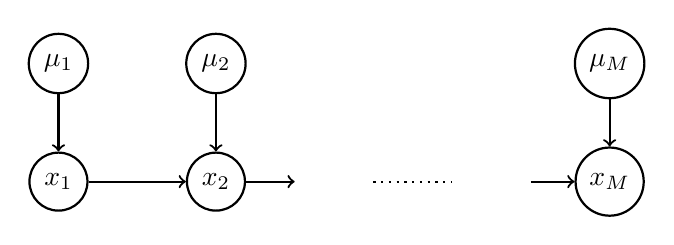
\begin{tikzpicture}
        % First pair
        \node[circle,draw=black,line width=0.8pt,minimum size=0.6cm] (mu1) at (0,1.5) {$\mu_1$};
        \node[circle,draw=black,line width=0.8pt,minimum size=0.6cm] (x1) at (0,0) {$x_1$};
        
        % Second pair
        \node[circle,draw=black,line width=0.8pt,minimum size=0.6cm] (mu2) at (2,1.5) {$\mu_2$};
        \node[circle,draw=black,line width=0.8pt,minimum size=0.6cm] (x2) at (2,0) {$x_2$};
        
        % Last pair
        \node[circle,draw=black,line width=0.8pt,minimum size=0.6cm] (muM) at (7,1.5) {$\mu_M$};
        \node[circle,draw=black,line width=0.8pt,minimum size=0.6cm] (xM) at (7,0) {$x_M$};
        
        % Vertical connections
        \draw[->,black,line width=0.8pt] (mu1) -- (x1);
        \draw[->,black,line width=0.8pt] (mu2) -- (x2);
        \draw[->,black,line width=0.8pt] (muM) -- (xM);
        
        % Horizontal connections with spaced ellipsis
        \draw[->,black,line width=0.8pt] (x1) -- (x2);
        \draw[->,black,line width=0.8pt] (x2) -- (3,0);
        \draw[dotted, black,line width=0.8pt] (4,0) -- (5,0);
        \draw[->,black,line width=0.8pt] (6,0) -- (xM);
      \end{tikzpicture}
      \caption{} 
      \label{fig:dir_prior}
    \end{figure}

    We could also choose to share a common prior over the parameters, trading flexibility for computational feasibility. 

    \begin{figure}[H]
      \centering 
      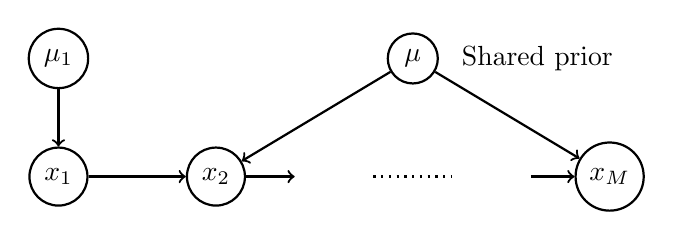
\begin{tikzpicture}
        % First mu node with x1
        \node[circle,draw=black,line width=0.8pt,minimum size=0.6cm] (mu1) at (0,1.5) {$\mu_1$};
        \node[circle,draw=black,line width=0.8pt,minimum size=0.6cm] (x1) at (0,0) {$x_1$};
        
        % Second x node
        \node[circle,draw=black,line width=0.8pt,minimum size=0.6cm] (x2) at (2,0) {$x_2$};
        
        % Last x node
        \node[circle,draw=black,line width=0.8pt,minimum size=0.6cm] (xM) at (7,0) {$x_M$};
        
        % Shared mu node
        \node[circle,draw=black,line width=0.8pt,minimum size=0.6cm] (mu) at (4.5,1.5) {$\mu$};
        
        % Label for shared prior
        \node[right] at (5,1.5) {Shared prior};
        
        % Vertical connections
        \draw[->,black,line width=0.8pt] (mu1) -- (x1);
        \draw[->,black,line width=0.8pt] (mu) -- (x2);
        \draw[->,black,line width=0.8pt] (mu) -- (xM);
        
        % Horizontal connections with spaced ellipsis
        \draw[->,black,line width=0.8pt] (x1) -- (x2);
        \draw[->,black,line width=0.8pt] (x2) -- (3,0);
        \draw[dotted, black,line width=0.8pt] (4,0) -- (5,0);
        \draw[->,black,line width=0.8pt] (6,0) -- (xM);
      \end{tikzpicture}
      \caption{} 
      \label{fig:shared_dir_prior}
    \end{figure}
  \end{example}

  Another way to make more compact representations is through parameterized models. For example, if we have to compute $p(y = 1 \mid \mathbf{x}_1, \ldots, \mathbf{x}_M)$, this in general has $O(K^M)$ parameters. However, we can obtain a more parsimonious form by using a logistic function acting on a linear combination of the parent variables 
  \begin{equation}
    p(y = 1 \mid \mathbf{x}_1, \ldots, \mathbf{x}_m) = \sigma \bigg( w_0 + \sum_{i=1}^M w_i x_i \bigg) = \sigma(\mathbf{w}^T \mathbf{x})
  \end{equation}
  We can look at an example how this is applied to sampling from high-dimensional Gaussian with \textbf{linear Gaussian models}.  


  \begin{example}[Multivariate Gaussian]
    Consider an arbitrary acyclic graph over $D$ random variables, in which eachnode represents a single continuous Gaussian distribution with its mean given by a linear function of its parents. 
    \[p(x_i \mid \mathbf{pa}_i) = N \bigg( x_i \bigg| w_{ij} x_j + b_j, v_i \bigg) \]
    Given a multivariate Gaussian, let us try to decompose it into a directed graph. The log of the joint distribution takes form 
    \[\ln p(\mathbf{x}) = \sum_{i=1}^D \ln p(x_i \mid \mathrm{pa}_i) = - \sum_{i=1}^D \frac{1}{2 v_i} \bigg( x_i - \sum_{j \in \mathrm{pa}_i} w_{ij} x_j - b_i \bigg)^2 + \mathrm{const}\]
    To compute the mean, we can see that by construction, every $x_i$ is dependent on its ancestors, so 
    \[x_i = \sum_{j \in \mathrm{pa}_i} w_{ij} x_j + b_i + \sqrt{v_i} \epsilon_i, \;\; \epsilon_i \sim N(0, 1)\]
    so by linearity of expectation, we have 
    \[\mathbb{E}[x_i] = \sum_{j \in \mathrm{pa}_i} w_{ij} \mathbb{E}[x_j] + b_i\]
    So again, we can start at the top of the graph and compute the expectation. To compute covariance, we can obtain the $i, j$th element of $\boldsymbol{\Sigma}$ with a recurrence relation: 
    \begin{align*} 
      \Sigma_{ij} & = \mathbb{E}[ (x_i - \mathbb{E}[x_i]) (x_j - \mathbb{E}[x_j])] \\
                  & = \mathbb{E} \bigg[ (x_i - \mathbb{E}[x_i]) \bigg( \sum_{k \in \mathrm{pa}_j} w_{j k} (x_k - \mathbb{E}[x_k])  + \sqrt{v_i} \epsilon_j\bigg) \bigg] \\
                  & = \sum_{k \in \mathrm{pa}_j} w_{j k} \Sigma_{ik} + I_{ij} v_j
    \end{align*}
    If there were no links in the graphs, then the $w_{ij}$'s are $0$, and so $\mathbb{E}[\mathbf{x}] = [b_1, \ldots, b_D]$, making the covariance diagonal.If the graph is fully connected, then the total number of parameters is $D + D(D-1)/2$, which corresponds to a general symmetric covariance matrix.  
  \end{example}

  \begin{example}[Bilinear Gaussian Model]
    Consider the following model
    \begin{align*}
      u & \sim N(0, 1) \\
      v & \sim N(0, 1) \\
      r & \sim N(u v, 1)
    \end{align*}
    where the mean of $r$ is a product of $2$ Gaussians. This is also a parameterized model. 

    \begin{figure}[H]
      \centering 
      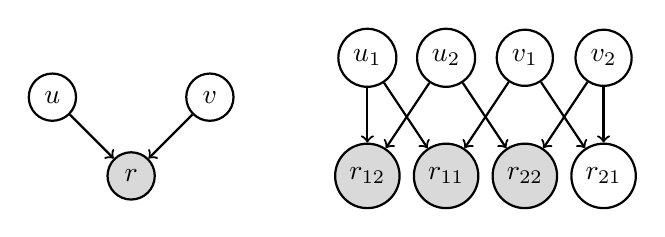
\begin{tikzpicture}
        % Left network
        \node[circle,draw=black,line width=0.8pt,minimum size=0.6cm] (u) at (-2,1) {$u$};
        \node[circle,draw=black,line width=0.8pt,minimum size=0.6cm] (v) at (0,1) {$v$};
        \node[circle,draw=black,line width=0.8pt,fill=gray!30,minimum size=0.6cm] (r) at (-1,0) {$r$};

        % Draw directed edges for left network
        \draw[->,black,line width=0.8pt] (u) -- (r);
        \draw[->,black,line width=0.8pt] (v) -- (r);

        % Right network
        \node[circle,draw=black,line width=0.8pt,minimum size=0.6cm] (u1) at (2,1.5) {$u_1$};
        \node[circle,draw=black,line width=0.8pt,minimum size=0.6cm] (u2) at (3,1.5) {$u_2$};
        \node[circle,draw=black,line width=0.8pt,minimum size=0.6cm] (v1) at (4,1.5) {$v_1$};
        \node[circle,draw=black,line width=0.8pt,minimum size=0.6cm] (v2) at (5,1.5) {$v_2$};
        
        \node[circle,draw=black,line width=0.8pt,fill=gray!30,minimum size=0.6cm] (r12) at (2,0) {$r_{12}$};
        \node[circle,draw=black,line width=0.8pt,fill=gray!30,minimum size=0.6cm] (r11) at (3,0) {$r_{11}$};
        \node[circle,draw=black,line width=0.8pt,fill=gray!30,minimum size=0.6cm] (r22) at (4,0) {$r_{22}$};
        \node[circle,draw=black,line width=0.8pt,minimum size=0.6cm] (r21) at (5,0) {$r_{21}$};

        % Draw directed edges for right network
        \draw[->,black,line width=0.8pt] (u1) -- (r12);
        \draw[->,black,line width=0.8pt] (u1) -- (r11);
        \draw[->,black,line width=0.8pt] (u2) -- (r12);
        \draw[->,black,line width=0.8pt] (u2) -- (r22);
        \draw[->,black,line width=0.8pt] (v1) -- (r11);
        \draw[->,black,line width=0.8pt] (v1) -- (r21);
        \draw[->,black,line width=0.8pt] (v2) -- (r22);
        \draw[->,black,line width=0.8pt] (v2) -- (r21);
      \end{tikzpicture}
      \caption{} 
      \label{fig:bilinear_gaussian}
    \end{figure}
  \end{example}

  \begin{definition}[Conditional Independence in Directed Graphs]
    We say that $a$ is independent of $b$ given $c$ if 
    \[p(a \mid b, c) = p(a \mid c)\]
    or equivalently, 
    \[p(a, b \mid c) = p(a \mid b, c)\, p(b \mid c) = p(a \mid c) \, p(b \mid c)\]
    Conveniently, we can directly read conditional independence properties of the joint distribution from the graph without any analytical measurements. 
  \end{definition}

  \begin{example}[Conditional Independence on Dataset]
    We can demonstrate conditional independence with iid data. Consider the problem of density estimation of some dataset $\mathcal{D} = \{x_i\}$ with some parameterized distribution of $\mu$. Originally, the observations are not independent since they depend on $\mu$. 
    \begin{equation}
      p(\mathcal{D}) = \int_{\mu} p(\mathcal{D} \mid \mu) \, p(\mu)\, d\mu 
    \end{equation}

    \begin{figure}[H]
      \centering 
      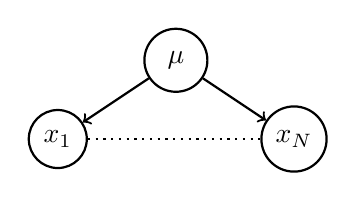
\begin{tikzpicture}
        \node[circle,draw=black,line width=0.8pt,minimum size=0.8cm] (mu2) at (0,-1) {$\mu$};
        
        \node[circle,draw=black,line width=0.8pt,minimum size=0.6cm] (x12) at (-1.5,-2) {$x_1$};
        \node[circle,draw=black,line width=0.8pt,minimum size=0.6cm] (xn2) at (1.5,-2) {$x_N$};
        
        \draw[->,black,line width=0.8pt] (mu2) -- (x12);
        \draw[->,black,line width=0.8pt] (mu2) -- (xn2);
        \draw[dotted,black,line width=0.8pt] (x12) -- (xn2);
      \end{tikzpicture}
      \caption{}
      \label{fig:conditional_indep_iid_1}
    \end{figure}

    If we condition on $\mu$ and considered the joint over the observed variables, the variables are independent. 
    \begin{equation}
      p(\mathcal{D} \mid \mu) = \prod_{n=1}^N p(x_n \mid \mu)
    \end{equation}

    \begin{figure}[H]
      \centering 
      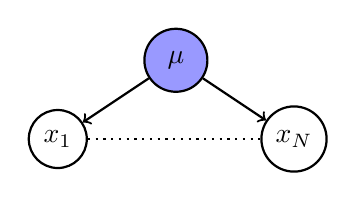
\begin{tikzpicture}
        \node[circle,draw=black,fill=blue!40,line width=0.8pt,minimum size=0.8cm] (mu1) at (0,2) {$\mu$};
        
        \node[circle,draw=black,line width=0.8pt,minimum size=0.6cm] (x11) at (-1.5,1) {$x_1$};
        \node[circle,draw=black,line width=0.8pt,minimum size=0.6cm] (xn1) at (1.5,1) {$x_N$};
        
        \draw[->,black,line width=0.8pt] (mu1) -- (x11);
        \draw[->,black,line width=0.8pt] (mu1) -- (xn1);
        \draw[dotted,black,line width=0.8pt] (x11) -- (xn1);
      \end{tikzpicture}
      \caption{}
      \label{fig:conditional_indep_iid_2}
    \end{figure}    
  \end{example}

  The example above identifies a node (the parent $\mu$) where, if observed, causes the rest of the nodes to become independent. We can extend on this idea by taking an arbitrary $x_i$ and finding a set of nodes such that if they are observed, then $x_i$ is indepedent from every other node. 

  \begin{definition}[Markov Blanket in Directed Graphs]
    The \textbf{Markov blanket} of a node is the minimal set of nodes that must be observed to make this node independent of all other nodes. It turns out that the parents, children, and coparents are all in the Markov blanket. 

    \begin{figure}[H]
      \centering 
      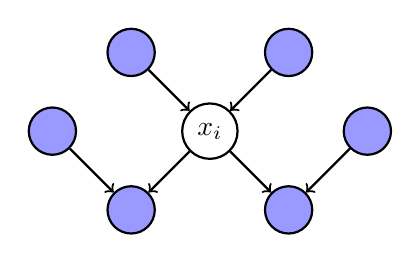
\begin{tikzpicture}
        % Central node
        \node[circle,draw=black,line width=0.8pt,minimum size=0.6cm] (c) at (0,0) {$x_i$};
        
        % Parent nodes (top)
        \node[circle,draw=black,fill=blue!40,line width=0.8pt,minimum size=0.6cm] (p1) at (-1,1) {};
        \node[circle,draw=black,fill=blue!40,line width=0.8pt,minimum size=0.6cm] (p2) at (1,1) {};
        
        % Middle level nodes
        \node[circle,draw=black,fill=blue!40,line width=0.8pt,minimum size=0.6cm] (m1) at (-2,0) {};
        \node[circle,draw=black,fill=blue!40,line width=0.8pt,minimum size=0.6cm] (m2) at (2,0) {};
        
        % Children nodes (bottom)
        \node[circle,draw=black,fill=blue!40,line width=0.8pt,minimum size=0.6cm] (c1) at (-1,-1) {};
        \node[circle,draw=black,fill=blue!40,line width=0.8pt,minimum size=0.6cm] (c2) at (1,-1) {};
        
        \draw[->,black,line width=0.8pt] (p1) -- (c);
        \draw[->,black,line width=0.8pt] (p2) -- (c);
        \draw[->,black,line width=0.8pt] (c) -- (c1);
        \draw[->,black,line width=0.8pt] (c) -- (c2);
        \draw[->,black,line width=0.8pt] (m1) -- (c1);
        \draw[->,black,line width=0.8pt] (m2) -- (c2);
      \end{tikzpicture}
      \caption{} 
      \label{fig:markov_blanket_directed}
    \end{figure} 

    Note that 
    \begin{equation}
      p(x_i \mid x_{j \neq i}) = \frac{p(x_1, \ldots, x_M)}{\int p(x_1, \ldots, x_M) \,dx} = \frac{\prod_k p(x_k \mid \mathrm{pa}_k)}{\int \prod_k p(x_k \mid \mathrm{pa}_k) \,dx_i}
    \end{equation}
  \end{definition} 

  One final interpretation is that we can view directed graphs as \textbf{distribution filters}. We take the joint probability distribution, will starts off as fully connected, and the directed graphs ``filters" away the edges that are not needed. Therefore, the joint probability distribution $p(\mathbf{x})$ is only allows through the filter if and only if it satisfies the factorization property. 

\subsection{Markov Random Field (Undirected Graphical Models)}

  As the name implies, undirected models use undirected graphs, which are used to model relationships that go both ways rather than just one. Unlike directed graphs, which are useful for expressing casual relationships between random variables, undirected graphs are useful for expressing soft constraints between random variables.  

  \begin{figure}[H]
    \centering 
    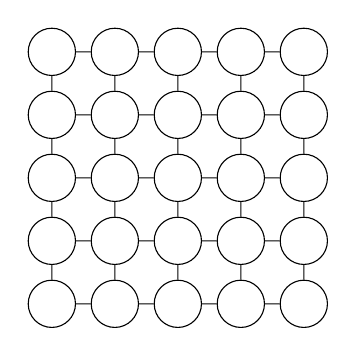
\begin{tikzpicture}[scale=0.8]
      \foreach \i in {1,...,5} {
        \foreach \j in {1,...,5} {
          \node[circle, draw, minimum size=0.6cm] (node\i\j) at (\i, \j) {};
        }
      }

      \foreach \i in {1,...,5} {
        \foreach \j in {1,...,5} {
          \pgfmathtruncatemacro{\right}{\i+1}
          \pgfmathtruncatemacro{\down}{\j-1}
          \pgfmathtruncatemacro{\up}{\j+1}
          \pgfmathtruncatemacro{\left}{\i-1}
          
          \ifnum \i < 5
            \draw (node\i\j) -- (node\right\j);
          \fi
          
          \ifnum \j > 1
            \draw (node\i\j) -- (node\i\down);
          \fi
        }
      }
    \end{tikzpicture}
    \caption{An MRF can be represented with this graph.} 
    \label{fig:mrf_graph}
  \end{figure}

  \begin{definition}[Conditional Independence in Undirected Graphs]
    Fortunately, conditional independence is easier compared to directed models. We can say $A$ is conditionally independent to $B$ given $C$ if $C$ blocks all paths between any node in $A$ and any node in $B$. 

    \begin{figure}[H]
      \centering 
      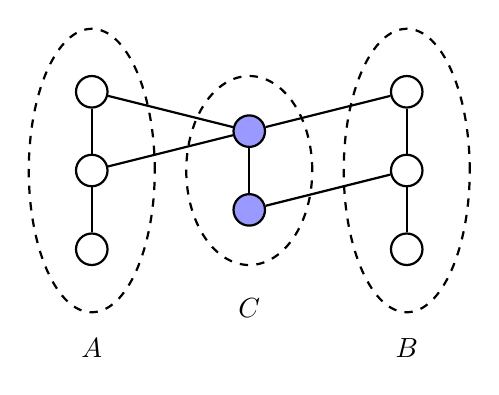
\begin{tikzpicture}
        \node[circle,draw=black,line width=0.8pt,minimum size=0.4cm] (a1) at (-2,1) {};
        \node[circle,draw=black,line width=0.8pt,minimum size=0.4cm] (a2) at (-2,0) {};
        \node[circle,draw=black,line width=0.8pt,minimum size=0.4cm] (a3) at (-2,-1) {};

        \node[circle,draw=black,line width=0.8pt,fill=blue!40,minimum size=0.4cm] (c1) at (0,0.5) {};
        \node[circle,draw=black,line width=0.8pt,fill=blue!40,minimum size=0.4cm] (c2) at (0,-0.5) {};

        % Right cluster (B)
        \node[circle,draw=black,line width=0.8pt,minimum size=0.4cm] (b1) at (2,1) {};
        \node[circle,draw=black,line width=0.8pt,minimum size=0.4cm] (b2) at (2,0) {};
        \node[circle,draw=black,line width=0.8pt,minimum size=0.4cm] (b3) at (2,-1) {};

        % Draw edges
        \draw[black,line width=0.8pt] (a1) -- (a2);
        \draw[black,line width=0.8pt] (a2) -- (a3);
        \draw[black,line width=0.8pt] (a1) -- (c1);
        \draw[black,line width=0.8pt] (a2) -- (c1);
        \draw[black,line width=0.8pt] (c1) -- (c2);
        \draw[black,line width=0.8pt] (c1) -- (b1);
        \draw[black,line width=0.8pt] (c2) -- (b2);
        \draw[black,line width=0.8pt] (b1) -- (b2);
        \draw[black,line width=0.8pt] (b2) -- (b3);

        % Draw dashed ellipses around clusters
        \draw[color={black},dashed,line width=0.8pt] (-2,0.0) ellipse (0.8cm and 1.8cm) node[below=2cm] {$A$};
        \draw[color={black},dashed,line width=0.8pt] (0,0) ellipse (0.8cm and 1.2cm) node[below=1.5cm] {$C$};
        \draw[color={black},dashed,line width=0.8pt] (2,0.0) ellipse (0.8cm and 1.8cm) node[below=2cm] {$B$};
      \end{tikzpicture}
      \caption{$A$ is conditionally independent given $C$, denoted $A \perp\!\!\!\perp B|C$. } 
      \label{fig:undirected_conditional_independence}
    \end{figure}
  \end{definition}

  \begin{definition}[Markov Blanket in Undirected Graphs]
    The Markov blanket of a node, which is the minimal set of nodes that must be observered to make this node independent of the rest of the nodes, is simply the nodes that are directly connected to that node. 

    \begin{figure}[H]
      \centering 
      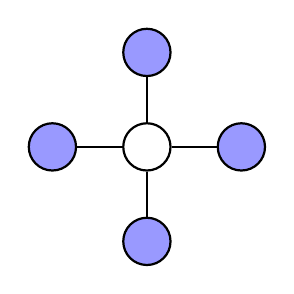
\begin{tikzpicture}
        % Central node
        \node[circle,draw=black,line width=0.8pt,minimum size=0.6cm] (c) at (0,0) {};
        
        % Filled outer nodes
        \node[circle,draw=black,fill=blue!40,line width=0.8pt,minimum size=0.6cm] (n1) at (0,1.2) {};
        \node[circle,draw=black,fill=blue!40,line width=0.8pt,minimum size=0.6cm] (n2) at (1.2,0) {};
        \node[circle,draw=black,fill=blue!40,line width=0.8pt,minimum size=0.6cm] (n3) at (0,-1.2) {};
        \node[circle,draw=black,fill=blue!40,line width=0.8pt,minimum size=0.6cm] (n4) at (-1.2,0) {};
        
        % Draw edges
        \draw[black,line width=0.8pt] (c) -- (n1);
        \draw[black,line width=0.8pt] (c) -- (n2);
        \draw[black,line width=0.8pt] (c) -- (n3);
        \draw[black,line width=0.8pt] (c) -- (n4);
      \end{tikzpicture}
      \caption{Once the neighbors of a node are realized, the node is independent of the rest of the nodes. } 
      \label{fig:markov_blanket_undirected}
    \end{figure}

    Therefore, the conditional distribution of $x_i$ conditioned on all the variables in the graph is dependent only on the variables in the Markov blanket. 
  \end{definition}

  Now, let us talk about how we can actually define a probability distribution with this graph. 

  \begin{definition}[Clique] 
    In an undirected graph, a \textbf{clique} is a set of nodes such that there exists a link between all pairs of nodes in that subset. A \textbf{maximal clique} is a clique such that it is not possible to include any other nodes in the set without it ceasing it to be a clique. 
  \end{definition}

  Given a joint random variable $\mathbf{x}$  represented by an undirected graph, the joint distribution is given by the product of non-negative potential functions over the maximal cliques 
  \begin{equation}
    p(\mathbf{x}) = \frac{1}{Z} \prod_C \phi_C (x_C)
  \end{equation}
  where 
  \begin{equation}
    Z = \int p(\mathbf{x}) \,d\mathbf{x}
  \end{equation}
  is the normalizing constant, called the \textbf{partition function}. That is, each $x_C$ is a maximal clique and $\phi_C$ is the nonnegative potential function of that clique. 

  This assignment looks pretty arbitrary. How do we know that any arbitrary joint distribution of $\mathbf{x}$, which has a undirected graphical representation, can be represented as the product of a bunch of functions over the maximum cliques? Fortunately, there is a mathematical result that proves this. 

  \begin{theorem}[Hammersley-Clifford] 
    The joint probability distribution of any undirected graph can be written as the product of potential functions on the maximal cliques of the graph. Furthermore, for any factorization of these potential functions, there exists an undirected graph for which is the joint.  
  \end{theorem} 


  \begin{example}
    For example, the joint distribution of the graph below
    \begin{figure}[H]
      \centering 
      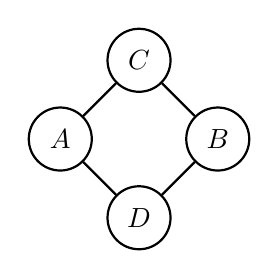
\begin{tikzpicture}
        % Define nodes
        \node[circle,draw=black,line width=0.8pt,minimum size=0.8cm] (A) at (-1,0) {$A$};
        \node[circle,draw=black,line width=0.8pt,minimum size=0.8cm] (B) at (1,0) {$B$};
        \node[circle,draw=black,line width=0.8pt,minimum size=0.8cm] (C) at (0,1) {$C$};
        \node[circle,draw=black,line width=0.8pt,minimum size=0.8cm] (D) at (0,-1) {$D$};

        % Draw thick edges
        \draw[black,line width=0.8pt] (A) -- (C);
        \draw[black,line width=0.8pt] (A) -- (D);
        \draw[black,line width=0.8pt] (B) -- (C);
        \draw[black,line width=0.8pt] (B) -- (D);
      \end{tikzpicture}
      \caption{} 
      \label{fig:hammersley_clifford_ex}
    \end{figure}
    factorizes into 
    \begin{equation}
      p(A, B, C, D) = \frac{1}{Z} \phi(A, C) \, \phi(C, B) \, \phi(B, D) \, \phi(A, D)
    \end{equation}
  \end{example}

  Note that each potential function $\phi$ is a mapping from the joint configuration of random variables in a clique to non-negative real numbers. The choice of potential functions is not restricted to having specific probabilistic interpretations, but since they must be nonnegative, we can just represent them as an exponential. The negative sign is not needed, but is a remnant of physics notation. 
  \begin{equation}
    p (\mathbf{x}) = \frac{1}{Z} \prod_C \phi_C (x_C) = \frac{1}{Z} \exp \bigg\{ - \sum_C E(x_C) \bigg\} = \frac{1}{Z} \underbrace{\exp \big\{ - E(\mathbf{x}) \big\}}_{\substack{\text{Boltzmann}\\ \text{distribution}}}
  \end{equation}

  Any distribution that can be represented as the form above is called a \textbf{Boltzmann distribution}. So far, all we stated is that the joint probability distribution can be expressed as the product of a bunch of potential functions, but besides the fact that it is nonnegative, there is no probabilistic interpretation of these potentials (or equivalently, the energy functions). While this does give us greater flexibility in choosing potential functions, we must be careful in choosing them (e.g. choosing something like $x^2$ may cause the integral to diverge, making the joint not well-defined).

  Clearly, these potential functions over the cliques should express which configuration of the local variables are preferred to others. It should assign higher values to configurations that are deemed (either by assumption or through training data) to be more probable. That is, each potential is like an ``expert" that provides some opinion (the value) on a configuration, and the product of the values of all the potential represents the total opinion of all the experts. Therefore, global configurations with relatively high probabilities are those that find a good balance in satisfying the (possibly conflicting) influences of the clique potentials. 

  \begin{example}[Transmission of Colds] 
    Say that you want to model a distribution over three binary variables: whether you or not you, your coworker, and your roommate is sick ($0$ represents sick and $1$ represents healthy). Then, you can make simplifying assumptions that your roommate and your coworker do not know each other, so it is very unlikely that one of thme will give the other an infection such as a cold directly. Therefore, we can model the indirect transmission of a cold from your coworker to your roommate by modeling the transmission of the cold from your coworker to you and then you to your roommate. Therefore, we have a model of form

    \begin{center}
      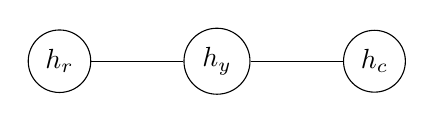
\begin{tikzpicture}
        \node[circle,draw] (hr) at (0,0) {$h_r$};
        \node[circle,draw] (hy) at (2,0) {$h_y$};
        \node[circle,draw] (hc) at (4,0) {$h_c$};

        \draw (hr) -- (hy);
        \draw (hy) -- (hc);
      \end{tikzpicture}
    \end{center}
    One max clique contains $h_y$ and $h_c$. The factor for this clique can be defined by a table and might have values resembling these. 

    \begin{table}[H]
      \centering
      \begin{tabular}{c|c|c|}
      \cline{2-3}
      & \( h_y = 0 \) & \( h_y = 1 \) \\ \hline
      \multicolumn{1}{|c|}{\( h_c = 0 \)} & 2 & 1 \\ \hline
      \multicolumn{1}{|c|}{\( h_c = 1 \)} & 1 & 10 \\ \hline
      \end{tabular}
      \caption{States and Values of \( h_y \) and \( h_c \)}
    \end{table}

    This table completely describes the potential function of this clique. Both of you are usually healthy, so the state $(1, 1)$ gets the maximum value of $1$. If one of you are sick, then it is likely that the other is sick as well, so we have a value of $2$ for $(0, 0)$. Finally, it is most unlikely that one of you is sick and the other healthy, which has a value of $1$. 
  \end{example}

\subsection{Hidden Markov Models}

